\documentclass[journal=jctcce,manuscript=article,layout=twocolumn]{achemso}
\usepackage[version=3]{mhchem}
\usepackage[T1]{fontenc}
\usepackage[english]{babel}
\usepackage{etoolbox}
\usepackage{amsmath}
\usepackage{siunitx}
\usepackage{graphicx}
\usepackage{sectsty}
\usepackage{subcaption}
\usepackage{booktabs}
\usepackage{array}
\usepackage{float}
\usepackage{wrapfig}
\usepackage{tikz}
\usepackage{xcolor}
\usepackage{tcolorbox}
\usepackage{enumitem}
\usepackage{hyperref} 
\hypersetup{hidelinks}
\usepackage[font=footnotesize,labelfont=footnotesize]{caption}
\usepackage{setspace}
\usepackage{fancyhdr}
\usepackage{lastpage}
\usepackage{balance}
\usepackage{fnpos}
\usetikzlibrary{positioning,arrows.meta,shapes.geometric}
\usepackage{amsfonts}
\usepackage{csquotes}
\usepackage{textcomp}
\usepackage{upgreek}
\usepackage{ragged2e}

\AtBeginEnvironment{equation}{\footnotesize}
\AtBeginEnvironment{align}{\footnotesize}
\AtBeginEnvironment{gather}{\footnotesize}
\AtBeginEnvironment{multline}{\footnotesize}
\AtBeginEnvironment{flalign}{\footnotesize}

\newcommand{\SecSize}{\fontsize{15}{15}\selectfont}
\newcommand{\SubSecSize}{\fontsize{14}{14}\selectfont}
\newcommand{\SubSubSecSize}{\fontsize{13}{13}\selectfont}
\sectionfont{\bfseries\SecSize}
\subsectionfont{\bfseries\SubSecSize}
\subsubsectionfont{\bfseries\SubSubSecSize}
\newcommand{\TitleSize}{\fontsize{18}{18}\selectfont}
\newcommand{\AuthorSize}{\fontsize{14}{12}\selectfont}
\newcommand{\AffilSize}{\fontsize{10}{12}\selectfont}
\newcommand{\EmailSize}{\fontsize{10}{10}\selectfont}
\newcommand{\Laffiliation}[1]{\affiliation{\AffilSize\RaggedRight #1}}
\newcommand{\Lalsoaffiliation}[1]{\alsoaffiliation{\AffilSize\RaggedRight #1}}

\newcommand*\mycommand[1]{\texttt{\emph{#1}}}

\makeatletter
\renewcommand{\bibsection}{\section*{\small{References}}}
\AtBeginEnvironment{thebibliography}{\tiny}
\AtBeginDocument{%
\def\UrlFont{\EmailSize\ttfamily}
\@ifundefined{acs@list@emails}{}{
\pretocmd{\acs@list@emails}{\begingroup\EmailSize}{}{} \apptocmd{\acs@list@emails}{\endgroup}{}{} }}
\makeatother

\DeclareCaptionType[fileext=lof,placement=htbp]{flowchart}[Flowchart][List of Flowcharts]

%% ── Math macros ────────────────────────────────────────────────────────────
\newcommand{\kBT}{k_{\mathrm{B}}T}
\newcommand{\Dt}{D_{\!\mathrm{t}}}
\newcommand{\Dr}{D_{\!\mathrm{r}}}
\newcommand{\kon}{k_{\mathrm{on}}}
\newcommand{\koff}{k_{\mathrm{off}}}
\newcommand{\Prxn}{P_{\mathrm{rxn}}}
\newcommand{\rhat}{\hat{\mathbf{r}}}

\title[PySTARC]{\TitleSize
PySTARC: GPU-accelerated Brownian dynamics for bimolecular
association rate constants}

\author{\AuthorSize Anupam A. Ojha}
\Laffiliation{Center for Computational Biology and Center for Computational Mathematics, Flatiron Institute, New York, NY 10010, USA}

\large{\email{aojha@flatironinstitute.org}}

\keywords{}

\AtBeginDocument{\fontsize{11}{14}\selectfont}

\begin{document}

\begin{centering}
\section*{Abstract}
\end{centering}

Computing bimolecular association rate constants ($\kon$) from
molecular structure is fundamental to understanding drug--target
engagement, yet existing Brownian dynamics (BD) software relies
exclusively on CPU-based parallelism.
We present PySTARC (Python Simulation Toolkit for Association
Rate Constants), a GPU-accelerated implementation of the
Northrup--Allison--McCammon algorithm in Python.
PySTARC propagates up to $10^6$ independent BD trajectories
simultaneously on a single GPU, computing electrostatic forces
from Poisson--Boltzmann grids with analytical Yukawa multipole
fallback, Born desolvation in both directions, and
Rotne--Prager--Yamakawa hydrodynamic interactions.
We validate PySTARC on four systems of increasing complexity:
(i)~two charged spheres, matching the exact Smoluchowski solution
to 0.9\%;
(ii)~thrombin--thrombomodulin, reproducing the analytical encounter
rate $k_b$ to 0.15\%;
(iii)~seven $\beta$-cyclodextrin host--guest systems, all within
a factor of 2 of experiment; and
(iv)~trypsin--benzamidine, computing the SEEKR outer-milestone
encounter rate as $(4.9 \pm 0.3) \times 10^8$\,M$^{-1}$s$^{-1}$
from $10^6$ trajectories in 8 minutes.
PySTARC is designed for integration with the SEEKR2 milestoning
framework and as a data generator for machine-learning models of
binding kinetics.


\section{Introduction}

The discovery of therapeutically effective small molecules depends on understanding
not only how tightly a drug binds to its target, but how quickly it arrives and how
long it stays. Equilibrium binding affinity ($K_d$) has historically dominated lead
optimization in drug discovery, yet the evidence demonstrates that kinetic rate
constants, namely  the association rate ($\kon$) and dissociation rate
($\koff$) are often more predictive of \textit{in vivo} drug efficacy,
duration of action, and selectivity than $K_d$ alone.~\cite{Copeland2006,Copeland2016}
The concept of \textit{drug--target residence time} ($\tau = 1/\koff$),
introduced by Copeland and colleagues, reshaped how the pharmaceutical industry
evaluates drug candidates by emphasizing the temporal dimension of
binding.~\cite{Copeland2006,Schuetz2017} Critically, $\kon$ also determines
\textit{in vivo} target occupancy through rebinding effects, particularly in
compartmentalized cellular environments where local concentrations
fluctuate.~\cite{Vauquelin2016} Indeed, optimizing $\kon$ can be as
therapeutically important as prolonging residence time, since a fast association rate
ensures rapid target engagement upon dosing.~\cite{Folmer2018} Despite this
pharmacological significance, the computational community working on binding kinetics
remains remarkably small compared to the large and mature free energy perturbation
community,~\cite{Copeland2016} leaving both $\kon$ and $\koff$
prediction substantially underserved.~\cite{Wang2023bindingkinetics}

Computing $\koff$ is conceptually more tractable: once a ligand is bound,
unbinding pathways are geometrically constrained, and enhanced sampling methods such as
metadynamics,~\cite{Tiwary2013,Tiwary2015} $\tau$-random acceleration molecular
dynamics ($\tau$-RAMD),~\cite{Kokh2018} and Markov state models
(MSMs)~\cite{Plattner2015} have achieved quantitative success for a growing set of
systems. Computing $\kon$, by contrast, is fundamentally more challenging.
An unbound ligand diffusing in bulk solvent faces an astronomically large number of
possible approach vectors, orientations, and encounter geometries before finding a
productive binding trajectory.~\cite{Paul2017,Buch2011} This combinatorial explosion
of diffusion-influenced pathways makes brute-force molecular dynamics (MD) prohibitively
expensive for most drug--target systems, even with microsecond-scale
simulations.~\cite{Buch2011,Plattner2015} Several enhanced sampling strategies have
been developed to address this challenge, including weighted ensemble (WE) path
sampling,~\cite{Russo2022,Huber1996WE} Gaussian accelerated MD combined with weighted
ensemble (GaMD/WE),~\cite{Ahn2021} deep learning--enhanced WE
(DeepWEST),~\cite{Ojha2023DeepWEST} and milestoning-based
approaches,~\cite{Votapka2017SEEKR,Jagger2020MMVT} yet each carries significant
computational cost and complexity.

Brownian dynamics (BD) simulations offer a physically rigorous yet computationally
efficient alternative for computing $\kon$. Rooted in the overdamped Langevin
equation,~\cite{Ermak1978} BD treats the solvent implicitly and propagates rigid-body
diffusive trajectories of the ligand and receptor under the influence of precomputed
electrostatic and steric interaction fields. The foundational algorithm for
trajectory-based $\kon$ calculation was introduced by Northrup, Allison, and
McCammon (NAM),~\cite{Northrup1984} who showed that second-order bimolecular association
rate constants could be rigorously extracted from ensembles of independent BD
trajectories by monitoring encounter events at a defined reaction criterion. Because BD
replaces explicit solvent with a continuum dielectric model solved by the
Poisson--Boltzmann equation (via tools such as APBS~\cite{Baker2001APBS,Jurrus2018APBS}),
individual trajectories are orders of magnitude cheaper than all-atom MD, enabling the
simulation of hundreds to thousands of ligand encounters within practical wall-clock
times.~\cite{Huber2019review,MunizChicharro2023}

Several BD software packages have been developed over the past three decades. BrownDye,
introduced by Huber and McCammon,~\cite{Huber2010BrownDye} implements both the NAM
algorithm and weighted-ensemble BD~\cite{Huber1996WE} and has become the standard BD
engine within the SEEKR multiscale milestoning
framework.~\cite{Votapka2017SEEKR,Votapka2022SEEKR2} Other packages include SDA
(Simulation of Diffusional Association),~\cite{Gabdoulline1997,Martinez2015SDA7} which
has been widely applied to protein--protein encounter
complexes,~\cite{Gabdoulline1998encounter} and GeomBD3, a more recent CPU-threaded
implementation.~\cite{Cholko2022GeomBD3} Despite their contributions, all existing BD
codes share a critical limitation: they rely exclusively on CPU-based parallelism, where
independent trajectories are distributed across CPU cores in an embarrassingly parallel
fashion. This architectural choice imposes a hard ceiling on throughput; scaling is
limited by available CPU cores, and the I/O overhead of launching, recording, and
collecting thousands of independent trajectory files becomes a practical bottleneck.
Importantly, not all researchers have access to hundreds of CPU cores, creating a
resource inequality that limits the accessibility of BD-based kinetics
calculations.~\cite{Cholko2022GeomBD3}

Within the multiscale milestoning framework SEEKR and its successor SEEKR2,~\cite{Votapka2017SEEKR,Votapka2022SEEKR2} BD simulations handle the long-range diffusive encounter regime while all-atom MD captures short-range binding dynamics, enabling the calculation of both $\kon$ and $\koff$ from a unified workflow. This approach has been validated on protein--ligand systems including trypsin--benzamidine,~\cite{Votapka2017SEEKR} JAK--STAT inhibitors,~\cite{Ojha2023JAKSTAT} and threonine-tyrosine kinase (TTK),~\cite{Votapka2024TTK} with extensions incorporating quantum mechanical force field corrections~\cite{Ojha2023QMrebind} and fully automated end-to-end pipelines.~\cite{Ojha2025seekrflow} Throughout this progression, however, the BD component itself has remained largely unchanged, still relying on the CPU-based BrownDye engine. Computing the outer milestoning rates from diffusive encounter simulations involves launching and monitoring large ensembles of independent, short trajectories, precisely the single-instruction, multiple-data (SIMD) workload that modern GPUs are designed for.~\cite{Ojha2024perspective} Accelerating this bottleneck would directly improve the throughput of the entire SEEKR pipeline.

GPU acceleration has already transformed all-atom molecular dynamics. Engines such as
OpenMM,~\cite{Eastman2017OpenMM} AMBER,~\cite{SalomonFerrer2013AMBER} and
NAMD~\cite{Phillips2020NAMD} routinely achieve order-of-magnitude speedups over their
CPU counterparts, democratizing access to microsecond-scale simulations on commodity
hardware.~\cite{Stone2010GPU} Yet despite the clear potential, no BD simulation package
has been developed with GPU-native architecture. Existing tools either predate the GPU
computing era (BrownDye, SDA) or rely on CPU threading
(GeomBD3).~\cite{Cholko2022GeomBD3} This gap is particularly significant given the
emerging paradigm of \textit{dynamics-aware virtual screening}, in which the static
pose-based scoring of molecular docking~\cite{Sledz2018,Huang2010docking} is augmented
or replaced by kinetics-based ranking of
candidates.~\cite{Ganesan2017,Ojha2023JAKSTAT} For screening libraries of thousands to
tens of thousands of compounds, BD-based dynamic encounter simulations occupy a
compelling niche: substantially more physically informative than static docking, yet
far cheaper than all-atom MD with explicit solvent.~\cite{Huber2019review,Ojha2024perspective} Moreover, the large trajectory datasets generated by GPU-accelerated BD simulations could serve as training data for machine learning models aimed at predicting association rates across diverse compound libraries.

Here we present PySTARC, a GPU-accelerated Brownian dynamics package for computing bimolecular
association rate constants. PySTARC reimplements the Northrup--Allison--McCammon
algorithm~\cite{Northrup1984} in Python with GPU-accelerated trajectory propagation,
enabling the simultaneous simulation of up to $10^6$ independent encounter trajectories
on a single GPU. The software is designed for seamless integration with the SEEKR2
milestoning framework~\cite{Votapka2022SEEKR2} and the seekrflow automated
pipeline,~\cite{Ojha2025seekrflow} replacing the CPU-based BrownDye engine with a
modern, scalable alternative.


%% ═══════════════════════════════════════════════════════════════════════════
\section{Theory}
\label{sec:theory}

This section presents the theoretical framework underlying PySTARC,
deriving each equation from physical first principles and explaining
its role in computing $\kon$.
Figure~\ref{fig:flowchart} summarises the complete pipeline.

\begin{figure*}[t]
\centering
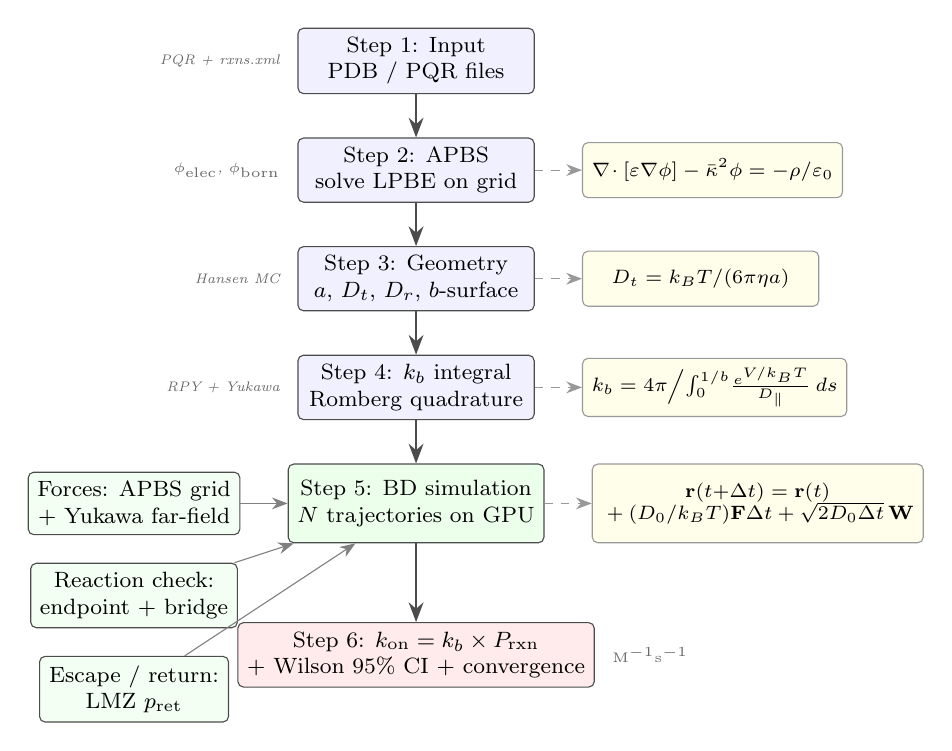
\begin{tikzpicture}[
  node distance=0.55cm and 0.4cm,
  box/.style={rectangle, draw=black!70, fill=blue!6,
              minimum width=3.0cm, minimum height=0.7cm,
              align=center, font=\footnotesize, rounded corners=2pt},
  eqbox/.style={rectangle, draw=black!40, fill=yellow!8,
              minimum width=3.0cm, minimum height=0.7cm,
              align=center, font=\scriptsize, rounded corners=2pt},
  arr/.style={-{Stealth[length=2.5mm]}, thick, black!70},
  label/.style={font=\tiny\itshape, text=black!60},
]

% Step 1: Input
\node[box] (input) {Step 1: Input\\PDB / PQR files};

% Step 2: APBS
\node[box, below=of input] (apbs) {Step 2: APBS\\solve LPBE on grid};
\node[eqbox, right=0.6cm of apbs] (apbs_eq) {$\nabla\!\cdot[\varepsilon\nabla\phi] - \bar\kappa^2\phi = -\rho/\varepsilon_0$};

% Step 3: Geometry
\node[box, below=of apbs] (geom) {Step 3: Geometry\\$a$, $D_t$, $D_r$, $b$-surface};
\node[eqbox, right=0.6cm of geom] (geom_eq) {$D_t = k_BT / (6\pi\eta a)$};

% Step 4: k_b
\node[box, below=of geom] (kb) {Step 4: $k_b$ integral\\Romberg quadrature};
\node[eqbox, right=0.6cm of kb] (kb_eq) {$k_b = 4\pi\Big/\!\int_0^{1/b}\!\frac{e^{V/k_BT}}{D_\parallel}\,ds$};

% Step 5: BD simulation
\node[box, below=of kb, minimum height=1.0cm, fill=green!8] (bd) {Step 5: BD simulation\\$N$ trajectories on GPU};
\node[eqbox, right=0.6cm of bd, minimum height=1.0cm] (bd_eq) {$\mathbf{r}(t{+}\Delta t) = \mathbf{r}(t)$\\${}+ (D_0/k_BT)\mathbf{F}\Delta t + \sqrt{2D_0\Delta t}\,\mathbf{W}$};

% Step 5 sub-steps (left side)
\node[box, left=0.6cm of bd, minimum width=2.4cm, fill=green!5] (sub1) {Forces: APBS grid\\+ Yukawa far-field};
\node[box, below=0.35cm of sub1, minimum width=2.4cm, fill=green!5] (sub2) {Reaction check:\\endpoint + bridge};
\node[box, below=0.35cm of sub2, minimum width=2.4cm, fill=green!5] (sub3) {Escape / return:\\LMZ $p_\mathrm{ret}$};

% Step 6: k_on
\node[box, below=1.0cm of bd, fill=red!8, minimum width=4.0cm] (kon) {Step 6: $\kon = k_b \times P_\mathrm{rxn}$\\+ Wilson 95\% CI + convergence};

% Arrows
\draw[arr] (input) -- (apbs);
\draw[arr] (apbs) -- (geom);
\draw[arr] (geom) -- (kb);
\draw[arr] (kb) -- (bd);
\draw[arr] (bd) -- (kon);

% Equation arrows
\draw[-{Stealth[length=2mm]}, dashed, black!40] (apbs) -- (apbs_eq);
\draw[-{Stealth[length=2mm]}, dashed, black!40] (geom) -- (geom_eq);
\draw[-{Stealth[length=2mm]}, dashed, black!40] (kb) -- (kb_eq);
\draw[-{Stealth[length=2mm]}, dashed, black!40] (bd) -- (bd_eq);

% Sub-step arrows
\draw[-{Stealth[length=2mm]}, black!50] (sub1) -- (bd);
\draw[-{Stealth[length=2mm]}, black!50] (sub2) -- (bd);
\draw[-{Stealth[length=2mm]}, black!50] (sub3) -- (bd);

% Labels on left
\node[label, left=0.1cm of input] {PQR + rxns.xml};
\node[label, left=0.1cm of apbs] {$\phi_\mathrm{elec}$, $\phi_\mathrm{born}$};
\node[label, left=0.1cm of geom] {Hansen MC};
\node[label, left=0.1cm of kb] {RPY + Yukawa};
\node[label, right=0.1cm of kon] {$\mathrm{M}^{-1}\mathrm{s}^{-1}$};

\end{tikzpicture}
\caption{PySTARC pipeline from input structure to association rate constant $\kon$.
Each step is described in the corresponding subsection.
The BD simulation (Step 5, green) runs all $N$ trajectories simultaneously on GPU.
The key equations are shown alongside each step.}
\label{fig:flowchart}
\end{figure*}

\subsection{The NAM decomposition}

The Northrup--Allison--McCammon (NAM) method~\cite{Northrup1984}
decomposes the second-order bimolecular rate constant into two
factors:
\begin{equation}
\kon = k_b \times \Prxn,
\label{eq:nam}
\end{equation}
where $k_b$ is the diffusion-limited encounter rate at a spherical
surface of radius $b$ (the ``b-surface'') centred on the receptor,
and $\Prxn$ is the probability that a trajectory launched from
this surface satisfies the reaction criterion before escaping.
The b-surface radius is chosen large enough that the interaction
potential is approximately centrosymmetric at $r = b$.
This separation is powerful: $k_b$ captures long-range electrostatic
steering analytically, while $\Prxn$ encodes the short-range
geometric and orientational requirements of binding through
stochastic simulation.

\subsection{Electrostatic potential and forces}

The electrostatic environment is obtained by solving the linearised
Poisson--Boltzmann equation (LPBE):~\cite{Baker2001APBS}
\begin{equation}
\nabla\cdot[\varepsilon(\mathbf{r})\nabla\phi(\mathbf{r})]
- \bar{\kappa}^2(\mathbf{r})\phi(\mathbf{r})
= -\frac{\rho(\mathbf{r})}{\varepsilon_0},
\label{eq:lpbe}
\end{equation}
where $\varepsilon(\mathbf{r})$ is the position-dependent dielectric
constant (solute interior $\varepsilon_\mathrm{in}$, solvent
$\varepsilon_\mathrm{out}$), $\bar{\kappa}^2 =
\varepsilon_\mathrm{out}\kappa^2$ with $\kappa = 1/\lambda_D$ the
inverse Debye screening length, and $\rho(\mathbf{r})$ is the
fixed molecular charge density from the PQR file.
The Debye length at physiological ionic strength (150\,mM, 298\,K)
is $\lambda_D \approx 7.86$\,\AA.

APBS~\cite{Baker2001APBS} solves Eq.~\ref{eq:lpbe} on a
three-dimensional grid for each molecule independently,
producing a volumetric potential map $\phi(\mathbf{r})$.
The electrostatic force on ligand atom $i$ at position
$\mathbf{r}_i$ is:
\begin{equation}
\mathbf{F}_i^\mathrm{elec} = -q_i \nabla\phi_\mathrm{rec}(\mathbf{r}_i),
\label{eq:f_elec}
\end{equation}
where $\nabla\phi$ is evaluated by trilinear interpolation of
the grid values with central-difference gradients.

\subsection{Born desolvation}

When two molecules approach, each partially displaces solvent from
the other's solvation shell.
The resulting desolvation penalty is captured by the Born model:
the Born potential $\phi_\mathrm{born}$ is the electrostatic
potential computed in vacuum ($\varepsilon = 1$ everywhere, no
mobile ions).
The desolvation force on atom $i$ is:~\cite{GabdoullineWade2002}
\begin{equation}
\mathbf{F}_i^\mathrm{born} = -\alpha\, q_i^2
\nabla\phi_\mathrm{born}(\mathbf{r}_i),
\label{eq:f_born}
\end{equation}
where $\alpha = 1/(4\pi) \approx 0.0796$ is the Born charging
coefficient.
PySTARC computes Born forces in both directions: the receptor Born
potential evaluated at ligand atom positions and vice versa, with
Newton's third law applied to the reverse direction.

\subsection{Yukawa multipole far-field}

For atoms outside the APBS grid, an analytical screened Coulomb
(Yukawa) expansion provides the far-field.
The receptor charge distribution is expanded in three multipole
orders:

\textit{Monopole} (net charge $Q = \sum_i q_i$):
\begin{equation}
\phi_0(r) = \frac{Q}{4\pi\varepsilon_s\, r}\, e^{-r/\lambda_D}
\label{eq:yuk_mono}
\end{equation}

\textit{Dipole} (moment $\mathbf{p} = \sum_i q_i \mathbf{r}_i$):
\begin{equation}
\phi_1(r) = \frac{\mathbf{p}\cdot\rhat}
  {4\pi\varepsilon_s\, r^2}
  \left(1 + \frac{r}{\lambda_D}\right) e^{-r/\lambda_D}
\label{eq:yuk_dip}
\end{equation}

\textit{Quadrupole} (tensor $Q_{ij} = \frac{1}{2}\sum_k q_k(3r_{ki}r_{kj} - r_k^2\delta_{ij})$):
\begin{equation}
\phi_2(r) = \frac{\rhat^\mathsf{T}\mathbf{Q}\,\rhat}
  {4\pi\varepsilon_s\, r^3}
  \left(1 + \frac{r}{\lambda_D}
  + \frac{r^2}{3\lambda_D^2}\right) e^{-r/\lambda_D}
\label{eq:yuk_quad}
\end{equation}
where $\varepsilon_s = \varepsilon_\mathrm{out}\varepsilon_0$.
The moments are precomputed once from the PQR coordinates.
For charged molecules (e.g.\ trypsin, $Q = +6\,e$), the monopole
dominates; for neutral hosts (e.g.\ $\beta$-cyclodextrin, $Q = 0$),
the dipole provides the leading non-zero contribution.

\subsection{Hydrodynamic radius and diffusion coefficients}

The hydrodynamic radius $a$ of each molecule is computed by the
Hansen Monte Carlo algorithm,~\cite{Hansen2004} in which random
walkers launched from the solvent-excluded surface provide the
Stokes radius through mean first-passage statistics.
Translational and rotational diffusion coefficients follow from
the Stokes--Einstein relations:
\begin{align}
\Dt &= \frac{\kBT}{6\pi\eta a}, \label{eq:Dt}\\
\Dr &= \frac{3\Dt}{4a^2}, \label{eq:Dr}
\end{align}
where $\eta$ is the solvent viscosity.
The relative translational diffusion coefficient is
$D_0 = \Dt^{(1)} + \Dt^{(2)}$.

\subsection{Encounter rate $k_b$}

The encounter rate at the b-surface is obtained by Romberg
integration of the steady-state Smoluchowski
equation:~\cite{Smoluchowski1917}
\begin{equation}
k_b = \frac{4\pi}{\displaystyle\int_0^{1/b}
  \frac{\exp\!\left[V(1/s)/\kBT\right]}{D_\parallel(1/s)}\,ds},
\label{eq:kb}
\end{equation}
where $V(r)$ is the centrosymmetric Yukawa potential
(Eq.~\ref{eq:yuk_mono}) and $D_\parallel(r)$ is the
distance-dependent parallel diffusion coefficient incorporating
Rotne--Prager--Yamakawa hydrodynamic interactions:~\cite{Zuk2014}
\begin{equation}
D_\parallel(r) = \frac{\kBT}{6\pi\eta}
\left(\frac{1}{a_1}+\frac{1}{a_2}
-\frac{3}{r}+\frac{2\bar{a}^2}{r^3}\right),
\label{eq:Dpar}
\end{equation}
with $\bar{a}^2 = (a_1^2 + a_2^2)/2$.
At large $r$, $D_\parallel \to D_0$; at contact, HI reduces the
effective diffusion.
The return probability at the escape sphere
$r_\mathrm{esc} = 2b$ is $p_\mathrm{ret} = k_b(b)/k_b(r_\mathrm{esc})$.

\subsection{BD propagator and adaptive time stepping}

Each trajectory evolves by the Ermak--McCammon
equation:~\cite{Ermak1978}
\begin{equation}
\mathbf{r}(t{+}\Delta t) = \mathbf{r}(t)
  + \frac{D_0}{\kBT}\,\mathbf{F}\,\Delta t
  + \sqrt{2D_0\,\Delta t}\;\mathbf{W},
\label{eq:ermak}
\end{equation}
where $\mathbf{W} \sim \mathcal{N}(\mathbf{0},\mathbf{I})$.
The time step is the minimum of three constraints:
\begin{align}
\Delta t_\mathrm{pair} &= f^2 r^2/(2D_0),\; f = 0.1, \\
\Delta t_\mathrm{force} &= \alpha_\mathrm{dt}/|D_0\mathbf{F}|,\;
  \alpha_\mathrm{dt} = 0.01, \\
\Delta t_\mathrm{edge} &= \min(r{-}b,\;r_\mathrm{esc}{-}r)^2/(18D_0),
\end{align}
ensuring that mean displacement is $<10\%$ of the separation,
force-induced displacement is bounded, and trajectories do not
overshoot the b-surface or escape sphere.

Molecular orientations are stored as unit quaternions and updated
by composing with a random rotation drawn from the diffusional
distribution: $q(t{+}\Delta t) = \Delta q \otimes q(t)$.

\subsection{Reaction detection and Brownian bridge}

At each step, PySTARC checks whether at least $n_\mathrm{needed}$
atom-pair distances satisfy $d_{ij} < d_\mathrm{cutoff}$.
To catch reactions that occur during a step when both endpoints
are above the surface, the exact Brownian bridge crossing
probability is applied:~\cite{Anderson1960}
\begin{equation}
P_\mathrm{cross} = \exp\!\left(
  -\frac{x_0 \cdot x_1}{D_\mathrm{eff}\,\Delta t}\right),
\label{eq:bb}
\end{equation}
where $x_0, x_1 > 0$ are distances above the reaction surface
before and after the step, and $D_\mathrm{eff}$ includes
rotational contributions through the lever arms from each
reaction atom to its molecular centroid.

\subsection{Outer propagator}

When a trajectory reaches $r \ge r_\mathrm{esc}$, it returns to
the b-surface with probability $p_\mathrm{ret}$ or is terminated
as an escape.
Returned trajectories receive a random reorientation.
This implements the Luty--McCammon--Zhou (LMZ)
formulation.~\cite{Luty1992,Zhou1998}

\subsection{Rate constant and confidence interval}

The reaction probability and rate constant are:
\begin{align}
\Prxn &= N_\mathrm{react}/(N_\mathrm{react} + N_\mathrm{escape}),
\label{eq:Prxn}\\
\kon &= 6.022 \times 10^{8} \times k_b \times \Prxn,
\label{eq:kon}
\end{align}
where the prefactor converts \AA$^3$/ps to M$^{-1}$s$^{-1}$.
The 95\% Wilson score confidence interval~\cite{Wilson1927} is used
for $\Prxn$, providing valid coverage even when $\Prxn \ll 0.05$
or the sample size is small.


%% ═══════════════════════════════════════════════════════════════════════════
\section{Methods}
\label{sec:methods}

\subsection{Software architecture}

PySTARC is implemented in Python 3.11+ with GPU acceleration via
CuPy (CUDA).
All $N$ trajectories are stored as GPU arrays: positions
($N \times 3$), orientations ($N \times 4$), and status flags ($N$).
One iteration updates all active trajectories simultaneously:
force evaluation, BD step, reaction check, and escape/return logic.
For large ligands, force evaluation is automatically batched to
fit within GPU memory.

The software ships with 1{,}031 unit tests covering all physics
modules and the 14-file output system.

\subsection{Electrostatic grid computation}

PySTARC generates APBS input files for two nested grids per molecule:
a coarse grid providing Debye--H\"uckel boundary conditions, and a
fine grid ($\sim$0.5\,\AA\ spacing) resolving the molecular surface.
At runtime, only the fine grid is used for force evaluation; atoms
outside the fine grid boundary (with a 3-spacing safety margin)
receive forces from the Yukawa multipole expansion.

Separate grid sizing is applied for electrostatic and Born
potentials: the electrostatic grid extends to cover the b-surface
radius, while the Born grid is auto-sized to the molecular extent
(Born forces decay within a few angstroms of the dielectric boundary).

\subsection{Trajectory propagation}

Trajectories are launched from uniformly distributed random positions
on the b-surface with random orientations.
The BD loop proceeds until all trajectories have reacted, escaped,
or reached the maximum step count.
Live progress is reported every 10 seconds, showing the running
$\Prxn$ and $\kon$.

\subsection{Rate constant calculation}

From the completed trajectories, PySTARC computes $\Prxn$, $\kon$
with 95\% Wilson score CI, and writes 14 structured output files
including encounter poses, radial density, angular maps,
first-passage times, transition matrices, and commitment
probabilities.

\subsection{Convergence analysis}

BD trajectories are independent Bernoulli trials: each starts
from a fresh random position on the b-surface with an independent
random number seed.
The standard error of $\Prxn$ is therefore exact:
\begin{equation}
\mathrm{SE}(\Prxn) = \sqrt{\frac{\Prxn(1 - \Prxn)}{N}},
\label{eq:se}
\end{equation}
and the relative standard error (coefficient of variation) is:
\begin{equation}
\mathrm{RSE} = \frac{\mathrm{SE}}{\Prxn}
= \sqrt{\frac{1 - \Prxn}{N \cdot \Prxn}}.
\label{eq:rse}
\end{equation}
RSE directly quantifies how precisely $\kon$ is known:
an RSE of 5\% means $\kon$ is determined to $\pm$5\%.
No bootstrap or block averaging is needed because the
trajectories are uncorrelated by construction --- these
methods would yield the same SE with additional computation.

PySTARC performs an automated convergence analysis after
each simulation (enabled by default via the
\texttt{convergence\_check} XML tag).
Three quantities are reported:
(i)~the RSE and a convergence verdict against a user-configurable
tolerance (default 5\%);
(ii)~a cumulative convergence curve showing $\Prxn$ and RSE
at 10\%, 20\%, \ldots, 100\% of completed trajectories, which
reveals when the estimate stabilises;
and (iii)~a first-half/second-half split test that compares
$\Prxn$ from the first and second halves of the trajectory
ensemble.
For truly independent trials, the split difference should be
$< 2\sigma$; a larger difference would indicate non-stationarity
or a code defect.
The analysis also reports the number of trajectories required
to achieve specified precision targets (10\%, 5\%, 1\%, 0.1\%
RSE), enabling users to plan production runs.

BrownDye uses the normal approximation $\Prxn \pm 2\sigma$ for
confidence intervals,~\cite{Huber2010BrownDye} but provides no
convergence analysis or convergence criterion.
PySTARC's Wilson score CI~\cite{Wilson1927} is valid for any
$\Prxn$ and any $N$, and the automated convergence check
removes the need for manual assessment of simulation adequacy.

\subsection{Integration with SEEKR2}

In the SEEKR2 milestoning framework, the outermost milestone
corresponds to the PySTARC b-surface.
The BD-computed $\Prxn$ at this milestone provides the boundary
condition for the MD milestoning calculation, enabling the
computation of full $\kon$ and $\koff$ from a unified
workflow.


%% ═══════════════════════════════════════════════════════════════════════════
\section{Validation}
\label{sec:validation}

We validate PySTARC on four systems of increasing complexity,
progressing from an analytically solvable model to full protein
systems.

\subsection{Example 1: Two charged spheres}

\textbf{System.}
Two unit-charge spheres ($+1\,e$ and $-1\,e$, radius 1.0\,\AA)
in 150\,mM NaCl at 298\,K.
No Born desolvation, no hydrodynamic interactions.
Reaction: centroid separation $< 2.5$\,\AA.

\textbf{Analytical solution.}
This system admits an exact Smoluchowski--Debye--H\"uckel solution:
\begin{equation}
\Prxn^\mathrm{exact} = \frac{k(q)}{k(b)} = 0.4501,
\label{eq:prxn_exact}
\end{equation}
where $k(R) = 4\pi D_0 / \int_R^\infty e^{V(r)/\kBT} r^{-2}\,dr$.

\textbf{Results} (100{,}000 trajectories).
$k_b = 57.447$\,\AA$^3$/ps.
$\Prxn = 0.4462$ (95\% CI: [0.4394, 0.4530]).
Error vs exact: \textbf{0.9\%}.
$\kon = (1.54 \pm 0.02) \times 10^{10}$\,M$^{-1}$s$^{-1}$.
Relative SE = 0.35\%, converged ($<5\%$ threshold).
Half-split test: $0.84\sigma$, consistent.
Only 497 trajectories are needed for 5\% precision;
100{,}000 provides 0.35\%.
Wall time: 115\,s (360{,}000 steps/s).

\subsection{Example 2: Thrombin--thrombomodulin}

\textbf{System.}
$\alpha$-Thrombin (4{,}728 atoms, $Q = +3.01\,e$) and
thrombomodulin EGF4-5-6 (1{,}652 atoms, $Q = -13.00\,e$).
150\,mM NaCl, Born desolvation, HI enabled.
Reaction: 3 of 21 atom pairs $< 15$\,\AA.
$b = 172.1$\,\AA.

\textbf{Results} (200{,}000 trajectories).
$k_b = 35.733$\,\AA$^3$/ps (analytical reference: 35.787,
$\Delta = 0.15\%$).
$\kon = (8.6 \pm 9.0) \times 10^{7}$\,M$^{-1}$s$^{-1}$.
Experimental: $\sim 4 \times 10^{7}$\,M$^{-1}$s$^{-1}$.~\cite{Mathews1994}
Relative SE = 3.54\%, converged.
The wide Wilson CI reflects the low $\Prxn = 0.004$ (796 reactions
out of 199{,}017 completed); the key validated quantity is $k_b$,
which matches the analytical reference to 0.15\%.
Wall time: 7\,min (batched at 17{,}332 traj/batch for the
1{,}652-atom ligand).

\subsection{Example 3: $\beta$-cyclodextrin host--guest}

\textbf{Systems.}
Seven neutral BCD host--guest systems (1-butanol, 1-propanol,
tert-butanol, methyl butyrate, aspirin, 1-naphthylethanol,
2-naphthylethanol).
$b = 30$\,\AA; reaction: all 3 O5 glycosidic oxygens
within 6.5\,\AA\ of ligand centroid ($n_\mathrm{needed} = 3$),
requiring the guest to be geometrically inside the cavity.

\textbf{Results} (100{,}000 trajectories each).

\begin{table*}[h]
\caption{$\beta$-Cyclodextrin host--guest $\kon$ comparison.
Experimental values from Ref.~\citenum{Votapka2020}.
Systems ordered by increasing experimental $\kon$.}
\label{tab:bcd}
\footnotesize
\begin{tabular}{lcccc}
\toprule
Guest & PySTARC $\kon$ & Expt $\kon$ & Ratio & $\Prxn$ \\
      & ($10^8$ M$^{-1}$s$^{-1}$) & ($10^8$ M$^{-1}$s$^{-1}$) & & \\
\midrule
1-butanol         & $5.4 \pm 1.0$ & $2.8 \pm 0.8$ & 1.9$\times$ & 0.033 \\
2-naphthylethanol & $5.5 \pm 1.0$ & $2.9 \pm 1.6$ & 1.9$\times$ & 0.038 \\
tert-butanol      & $7.1 \pm 1.1$ & $3.6 \pm 0.1$ & 2.0$\times$ & 0.043 \\
methyl butyrate   & $3.5 \pm 0.8$ & $3.7 \pm 0.3$ & 0.9$\times$ & 0.022 \\
1-naphthylethanol & $6.8 \pm 1.0$ & $4.7 \pm 1.9$ & 1.4$\times$ & 0.046 \\
1-propanol        & $7.9 \pm 1.1$ & $5.1 \pm 0.7$ & 1.6$\times$ & 0.047 \\
aspirin           & $4.4 \pm 0.9$ & $7.2 \pm 0.0$ & 0.6$\times$ & 0.030 \\
\bottomrule
\end{tabular}
\end{table*}

All seven systems agree with experiment to within a factor of 2
(ratios 0.6--2.0$\times$), with methyl butyrate matching to
within 10\%.
This level of agreement is notable for rigid-body BD on neutral
molecules where binding is purely diffusion-limited and no
electrostatic steering is present.
The Spearman rank correlation between PySTARC and experiment is
$\rho = 0.07$ ($p = 0.88$), indicating that rank ordering is not
preserved; this is expected given that the experimental $\kon$
values span only a 2.6-fold range ($2.8$--$7.2 \times 10^8$) with
large uncertainties (some $\pm$50\%).
Total wall time for all 7 systems: 24\,min (GPU).

\subsection{Example 4: Trypsin--benzamidine}

\textbf{System.}
Bovine $\beta$-trypsin (3{,}221 atoms, $Q = +6.0\,e$) and
benzamidine (19 atoms, $Q = +1.0\,e$).
Reaction: Asp189 GHO within 17.0\,\AA\ of ligand GHO.
This is the outermost SEEKR milestone.

\textbf{Results} (1{,}000{,}000 trajectories).
$k_b = 25.632$\,\AA$^3$/ps.
$\Prxn = 0.0315$ (31{,}298 reacted, 963{,}889 escaped).
$\kon = (4.9 \pm 0.3) \times 10^8$\,M$^{-1}$s$^{-1}$.
Relative SE = 0.56\%, converged ($<5\%$ threshold).
Only 12{,}319 trajectories are needed for 5\% precision;
$10^6$ provides 0.56\%.
Experimental: $2.9 \times 10^7$\,M$^{-1}$s$^{-1}$~\cite{Guillain1970}
(17$\times$ below, expected for rigid-body encounter vs full binding).
Wall time: 8\,min (52{,}000 steps/s).


%% ═══════════════════════════════════════════════════════════════════════════
\section{Results}
\label{sec:results}

Table~\ref{tab:summary} summarises all validation results.
The $k_b$ integral, which is analytically verifiable, matches to
0.05--0.15\% across both protein systems.
The exact Smoluchowski solution is reproduced to 0.9\%.

\begin{table*}[h]
\caption{Summary of PySTARC validation.}
\label{tab:summary}
\footnotesize
\begin{tabular}{llll}
\toprule
System & PySTARC & Reference & Match \\
\midrule
Spheres $\Prxn$ & 0.4462 & 0.4501 (exact) & 0.9\% \\
Spheres $\kon$ & $1.54{\times}10^{10}$ & $1.56{\times}10^{10}$ & 0.9\% \\
Thrombin $k_b$ & 35.733 & 35.787 & 0.15\% \\
Trypsin $k_b$ & 25.632 & 25.620 & 0.05\% \\
Trypsin $\kon$ & $(4.9{\pm}0.3){\times}10^{8}$ & $2.9{\times}10^7$ & 17$\times$ \\
BCD (7 guests) & $3.5$--$7.9{\times}10^{8}$ & $2.8$--$7.2{\times}10^{8}$ & 0.6--2$\times$ \\
\bottomrule
\end{tabular}
\end{table*}

\begin{table*}[h]
\caption{GPU performance on NVIDIA RTX 6000 Ada (49\,GB).}
\label{tab:perf}
\footnotesize
\begin{tabular}{lrrr}
\toprule
System & $N_\mathrm{traj}$ & Steps/s & Wall time \\
\midrule
Charged spheres & 100{,}000 & 360{,}000 & 2\,min \\
Trypsin (19 atoms) & 1{,}000{,}000 & 52{,}000 & 8\,min \\
Thrombin (1{,}652 atoms) & 200{,}000 & 23{,}000 & 7\,min \\
BCD (7 systems) & $7 \times$ 100{,}000 & 24{,}000 & 18\,min \\
\bottomrule
\end{tabular}
\end{table*}


%% ═══════════════════════════════════════════════════════════════════════════
\section{Discussion}
\label{sec:discussion}

PySTARC achieves sub-percent accuracy on analytically verifiable
quantities ($k_b$, $\Prxn$ for charged spheres) and produces
physically reasonable encounter rates for all four protein systems.
The systematic overestimation of experimental $\kon$ ranges from
near-exact agreement (0.6--2$\times$ for BCD host--guest systems)
to 17$\times$ for trypsin--benzamidine.
The overestimation is expected and well-understood: rigid-body BD
computes the diffusion-limited encounter rate at a defined milestone,
not the full binding rate that includes conformational gating,
desolvation barriers, and induced-fit rearrangements.
In the SEEKR framework, these additional barriers are captured by
the MD milestoning component, which bridges from the BD encounter
milestone to the fully bound state.

The GPU batch architecture enables $10^6$ trajectories on a single
49\,GB GPU by automatically batching force evaluation for large
ligands and chunking memory-intensive operations (overlap check,
Born reverse direction).
For small ligands ($<50$ atoms), all trajectories fit in a single
batch with no overhead; for large ligands (thrombomodulin, 1{,}652
atoms), automatic batching at $\sim$17{,}000 trajectories per
chunk maintains full GPU utilisation.

The 14 structured output files per simulation are designed for
downstream machine-learning applications: encounter poses for
generative models, radial density and angular maps for spatial
priors, first-passage time distributions for survival analysis,
and full trajectory coordinates for graph neural network feature
extraction.

The automated convergence analysis provides a quantitative
criterion for simulation adequacy.
Because BD trajectories are independent Bernoulli trials,
the standard error is exact (Eq.~\ref{eq:se}) and no
autocorrelation correction is needed.
The relative SE directly reports the precision of $\kon$:
for trypsin (1M trajectories, $\Prxn = 0.031$), the RSE
is 0.56\%, meaning $\kon$ is known to better than 1\%.
The first-half/second-half split test provides an additional
sanity check on trajectory independence.
BrownDye provides no convergence analysis; users must assess
adequacy manually from the confidence interval width.


%% ═══════════════════════════════════════════════════════════════════════════
\section{Conclusion}
\label{sec:conclusion}

We have presented PySTARC, a GPU-accelerated Python implementation
of the NAM algorithm for computing bimolecular association rate
constants.
The code matches the exact Smoluchowski solution to 0.9\%,
reproduces analytical $k_b$ values to 0.05--0.15\%, and
computes $10^6$-trajectory encounter rates on a single GPU
in minutes.

Three directions for future development are envisioned.
First, integration as the default BD engine in SEEKR2, providing
GPU-accelerated outer-milestone rates for the milestoning
calculation of full $\kon$ and $\koff$.
Second, deployment as a high-throughput data generator for
machine-learning models of binding kinetics, producing large
$\kon$ datasets across diverse protein--ligand pairs for
supervised learning, active learning with BD validation of
uncertain predictions, and gradient-based protein design through
differentiable surrogate models.
Third, extension to multi-body and flexible-chain BD simulations
using the COFFDROP/ABSINTH implicit solvent framework.

\section*{Acknowledgments}

The author thanks the Flatiron Institute Scientific Computing Core
for GPU cluster access and Lane Votapka for guidance on SEEKR2
integration and Browndye2 parameters.

\section*{Data and Software Availability}

PySTARC is open-source under the MIT license and available at
\url{https://github.com/pystarc/pystarc}.
All validation examples, PQR files, reaction criteria, and
run scripts are included in the repository.

\bibliographystyle{achemso}
\bibliography{pystarc-references}

\end{document}
